\documentclass[11pt]{article}
\usepackage{xltxtra}
\usepackage{bookmark}
\usepackage{hyperref}
\hypersetup{hidelinks}
\usepackage{url}
\urlstyle{tt}
\usepackage{multicol}
\usepackage{xcolor}
\usepackage{calc}
\usepackage{graphicx}
\usepackage{tikz}
\usetikzlibrary{calc}
\usepackage{fontspec}
\usepackage{xeCJK}
\usepackage{relsize}
\usepackage{xspace}
\usepackage{fontawesome5}
\usepackage{titlesec}
\usepackage{enumitem}
\usepackage{siunitx}
\usepackage{amssymb}
\usepackage{tabularx}
\usepackage{multicol}
\usepackage{fontspec}
\usepackage{fancybox}
\usepackage{float}

% 取消中文字符与数字之间的间隔
\CJKsetecglue{}
\protected\def\Cpp{{C\nolinebreak[4]\hspace{-.05em}\raisebox{.28ex}{\relsize{-1}++}}\xspace}
\setlength{\parindent}{0pt}
\pagenumbering{gobble}
\setlist[itemize]{topsep=0em, leftmargin=*}
\setlist[enumerate]{topsep=0em, leftmargin=*}

% ========== 标题格式设置（改为黑体） ==========
% 一级标题：黑体，大号，加粗
\titleformat{\section}
{\LARGE\bfseries\sffamily\raggedright}  % \sffamily 使用无衬线字体（黑体）
{}{0em}
{}
[{\color{WHU_Blue}\titlerule}]
\titlespacing*{\section}{0cm}{*1}{*1}

% 二级标题：黑体，较大，加粗
\titleformat{\subsection}
{\large\bfseries\sffamily\raggedright}  % \sffamily 使用无衬线字体（黑体）
{}{0em}
{}
[]
\titlespacing*{\subsection}{0cm}{*1}{*1}

\usepackage[
a4paper,
left=1.2cm,
right=1.2cm,
top=1.5cm,
bottom=1cm,
nohead
]{geometry}

\renewcommand{\arraystretch}{1.2}
\linespread{1.2}
\renewcommand{\CJKglue}{\hskip 0.05em}

% ========== 字体设置 ==========
% 英文字体：Times New Roman（正文）
% 中文字体：宋体（正文）
% 标题字体：黑体（通过 \sffamily 实现）

% 设置英文字体（明确指定粗体）
\setmainfont{Times New Roman}[
BoldFont = Times New Roman Bold,
ItalicFont = Times New Roman Italic,
BoldItalicFont = Times New Roman Bold Italic,
]

% 设置无衬线字体（用于标题）
\setsansfont{Arial}[
BoldFont = Arial Bold,
]

% 设置等宽字体
\setmonofont{Courier New}[
BoldFont = Courier New Bold,
]

% 设置中文字体（明确指定粗体）
\setCJKmainfont{SimSun}[
BoldFont = SimHei,        % 宋体的粗体用黑体代替
ItalicFont = SimSun,      % 宋体通常没有斜体
]

% 设置中文无衬线字体（用于标题）
\setCJKsansfont{SimHei}[
BoldFont = SimHei,         % 黑体本身就有粗体效果
]

% 设置中文等宽字体
\setCJKmonofont{FangSong}[
BoldFont = SimHei,         % 仿宋的粗体用黑体代替
]

% 自定义主题色
\definecolor{WHU_Blue}{RGB}{0, 37, 84}

% 减小 itemize 间距
\setlist[itemize]{topsep=0pt, partopsep=0pt, parsep=0pt, itemsep=2pt, leftmargin=*}

% 填写个人信息
% 学院
\newcommand{\school}{乐育书院丨Leyu College} 

% 联系方式
\newcommand{\contact}{
	\scriptsize
	\textcolor{white}{
		\faEnvelope \quad \href{mailto:202411079123@mail.bnu.edu.com}{202411079123@mail.bnu.edu.cn}
		\hspace{4em}
		\faPhone \quad  134-3088-6102
	}
}

%%%%%%%%%%%%%%%%%%%%
% 简历正文
%%%%%%%%%%%%%%%%%%%%
\begin{document}
	% 页眉：校标组合+学院名
	\begin{tikzpicture}[remember picture, overlay]
		\node[anchor=north, inner sep=0pt](header) at (current page.north){
			
\includegraphics[width=\paperwidth]{images/header.png}
		};
		% 左边校徽
		\node[anchor=west](school_logo) at (header.west){
			\hspace{0.5cm}
			
\includegraphics[width=0.2\textwidth]{images/北京师范大学校徽校名白色.png}
		};
		% 右边乐育书院图标
		\node[anchor=east](school_name) at(header.east){
			\hspace{0.5cm}
			
\includegraphics[width=0.15\textwidth]{images/乐育书院.png}
			\hspace{0.5cm}
		};
	\end{tikzpicture}
	\vspace{-3.5em}
	
	% 页脚，联系方式
	\begin{tikzpicture}[remember picture, overlay]
		\node[anchor=south, inner sep=0pt](footer) at (current page.south){
			
\includegraphics[width=\paperwidth]{images/footer.png}
		};
		% 联系方式
		\node[anchor=center] at(footer.center){\contact};
	\end{tikzpicture}
	
	% 背景
	\begin{tikzpicture}[remember picture, overlay]
		\node[opacity=0.05] at(current page.center){
			
\includegraphics[width=0.7\paperwidth, keepaspectratio]{images/bnu_logo_big.png}
		};
	\end{tikzpicture}
	
	% 个人信息
	\begin{figure}[h]
		% 左半边，信息
		\begin{minipage}{0.82\textwidth}
			\vspace*{-25pt}
			\section{\makebox[\widthof{\faAddressCard}][c]{\color{WHU_Blue}{\faAddressCard}}\quad 个人信息}
			\begin{tabularx}{\linewidth}{p{\widthof{出生日期:}}Xp{\widthof{政治面貌:}}X}
				姓\ \ \ \ \ \ \ \ 名: & 石继楷 & 
				出生年月: & 2006年4月  \\
				邮\ \ \ \ \ \ \ \ 箱: & 202411079123@mail.bnu.edu.cn & 
				求职意向: & 数学教师 \\
			\end{tabularx}
		\end{minipage}
		\hspace{2em}
		% 右半边，照片
		\vspace*{-10pt}
		\begin{minipage}{0.12\textwidth}
			\setlength{\fboxsep}{0pt}
			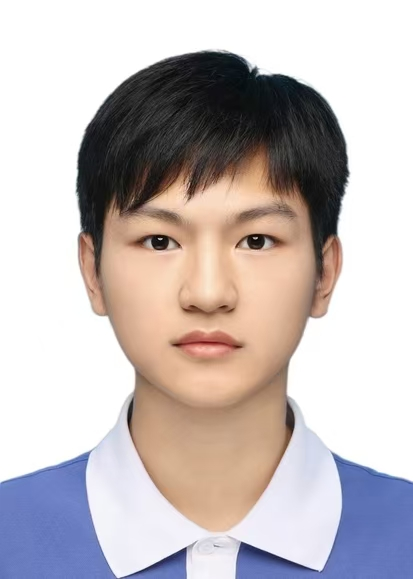
\includegraphics[width=\linewidth]{images/证件照.jpg}
		\end{minipage}
	\end{figure}
	\vspace{-1em}
	\vspace*{-25pt}
	% 教育背景
	\section{\makebox[\widthof{\faGraduationCap}][c]{\color{WHU_Blue}{\faGraduationCap}}\quad 教育背景}
	
	% 教育背景（本科生）
	{\large \textbf{北京师范大学}} \hspace{1.4cm} \textbf{硕士研究生} \hspace{1.6cm} \textbf{学科教学（数学）} \hfill {2028年9月 - 2030年7月} 
	
	\begin{itemize}
		
		% \item \href{学院官网.whu.edu.cn}{\underline{自强学堂}}，专业：你的专业  
		\item \textbf{主修课程}：数学课程与教材分析、数学教学设计与案例分5析、数学教育测量与评价、中学数学解题研究\ 等。
	\end{itemize}
	\vspace{0.5em}
	{\large \textbf{北京师范大学}} \hspace{1.9cm} \textbf{本科} \hspace{1.5cm} \textbf{数学与应用数学（公费师范）} \hfill 2024年9月 - 2028年7月
	
	\begin{itemize}
		
		\item \textbf{主修课程}：数学分析（83）、常微分方程（91）、教育学（89）、现代教育技术（94）、Python（96）\ 等。
		\item \textbf{担任职务}：\textbf{乐育书院团委组织部干事}（整理学生团籍资料，审核实践报销材料，担任入团考试、表彰大会场务 等）、乒乓球社团副社长、\textbf{班级宣传委员}（发表推文十余篇）、全媒体宣传中心文字采编部干事
		\item \textbf{所获荣誉}：\textbf{京师三等奖学金}，\textbf{学业二等奖学金}
	%	\item \textbf{GPA}：3.4 / 4.0（排名30 / 70）
	\end{itemize}
	
	\vspace{0.5em}
	{\large \textbf{深圳市第二高级中学}}\hfill 2021年9月 - 2024年7月
	
	\begin{itemize}
	\item 班级第一、多次超越奖，\textbf{总分年级第21}%，高考616
	\end{itemize}
	
	\vspace{-10pt}
		% 实践经历
	\section{\makebox[\widthof{\faGraduationCap}][c]{\color{WHU_Blue}{\faUniversity}}\quad 实践经历}
%	\textbf{教育实习}
	\begin{itemize}
		\item \textbf{贵州省沿河土家族自治县第二高级中学} \hfill 2025年6月 - 2025年7月\\
		在两周的暑期教育实践中，担任实习数学教师与班主任，累计授课5节，独立完成5份教案撰写、2次单元测验组织及60+份试卷批改
	%	\item \textbf{深圳市石厦学校} \hfill 2027年9月 - 2027年12月\\
	%	在一学期教育见习中担任实习数学教师与班主任，累计授课40+节；独立完成12份教案撰写、4次单元测验组织及300+份试卷批改，班级数学平均分较学期初提升6分
		%\item \textbf{京海小学}（202X年7月）担任支教队数学科组长，设计了《数学之美》系列课程
		\item \textbf{援藏“云陪伴”志愿服务} \hfill 2026年3月 - 2026年8月\\
		教授五年级下学期课程20节，形成“彩云之桥云伴学志愿者记录”、“学生成长手册”
	\end{itemize}
	
	
	\vspace{-10pt}
	% 获奖情况
	\section{\makebox[\widthof{\faGraduationCap}][c]{\color{WHU_Blue}{\faTrophy}}\quad 获奖情况}
		
		\textbf{全国大学生数学建模竞赛省部级三等奖} \hfill 2025年9月
		\begin{itemize}
			\item 负责建模、编程、论文撰写任务
			\item 针对孕妇及胎儿检测核心问题，对 NIPT（无创产前检测）相关数据建模分析
			\item 构建线性混合效应模型、改进 Canopy-Kmeans 聚类算法、CART 决策树等模型，完成胎儿 Y 染色体浓度相关性分析、分组最佳检测时点确定及女胎异常判定，最终形成完整建模报告，获省部级三等奖
		\end{itemize}
		
		\textbf{全国大学生数学竞赛（数学A类）省部级三等奖} \hfill 2025年11月%9日
		\begin{itemize}
			\item 聚焦解析几何、线性代数、数学分析等核心考点，独立完成六道竞赛题目解答
			\item 攻克向量运算、线性算子、积分不等式证明等重难点模块
		\end{itemize}	
		
		
		\textbf{“绿竹”班主任技能大比武二等奖} \hfill 2025年12月%7日
		\begin{itemize}
			\item 参与设计带班育人方略与主题班会设计
			\item 代表团队进行“3分钟情景模拟”，准确、快速拆解家校沟通问题情景的根本原因，高效完成现场应答
		\end{itemize}
		
		\textbf{第三届师范生文化节\textbf{板书设计大赛二等奖}、\textbf{教案设计大赛三等奖}、\textbf{最美三笔字评比三等奖}}\hfill 2025年3月
		\begin{itemize}
			\item 以“空间向量与立体几何”为主题的板书设计以及对应复习课教案分别获得二等奖与三等奖
			\item 粉笔字作品《无题》在三笔字的粉笔字赛道获得三等奖
		\end{itemize}

	% 工作技能
	\vspace*{-10pt}
	\section{\makebox[\widthof{\faGraduationCap}][c]{\color{WHU_Blue}{\faWrench}}\quad 专业技能}
	\begin{itemize}
	%	\item 教师资格证：高中数学，合格
		\item 普通话二级甲等、CET6成绩507分
		\item 熟练使用Office办公软件，以及LaTeX（建模常用）、MATLAB、Maple、VScode（编写c语言、python代码）等专业技能软件
	%	\item 编程：Matlab，Python，c
	\end{itemize}
	
\end{document}